\chapter{Metodologia}
\label{ch:metodologia}

\section{Unidade funcional e alternativas comparadas}
\label{sec:unidade-funcional}

A unidade funcional adotada neste trabalho é o movimento da mesma remessa de carga conteinerizada entre a mesma origem e o mesmo destino no Brasil. A remessa é caracterizada por uma massa de carga e, quando aplicável, por uma base em TEU. Essa definição fixa o serviço logístico a ser atendido antes da escolha modal: o que se compara não é um caminhão contra um navio em abstrato, mas duas cadeias alternativas para atender ao mesmo par origem-destino.

A primeira cadeia é a alternativa rodoviária direta. Nela, a carga percorre uma única perna rodoviária entre origem e destino, e os totais de distância, custo modelado e emissões são atribuídos a essa perna. A segunda cadeia é a alternativa rodoviária-cabotagem-rodoviária. Nela, a carga percorre um acesso rodoviário inicial até o porto de origem (\emph{pre-carriage}), uma perna marítima de cabotagem, componentes portuários e de \emph{hoteling} quando incluídos na fronteira do cenário, e um acesso rodoviário final do porto de destino até o destino da carga (\emph{on-carriage}) \cite{shortsea2019,competitiveness2024,modalshiftreview2020}.

Nos artefatos de validação e sensibilidade deste TF, a base recorrente é \texttt{1 TEU / 14 t} por remessa. Essa base organiza a comparação acadêmica realizada no relatório, mas não é apresentada como valor universal para todo uso futuro do \CabotageLens{}. Qualquer normalização por tonelada, TEU, contêiner ou tonelada-quilômetro só é interpretável quando preserva a carga, a distância, a regra de alocação e as fronteiras ambiental e econômica do cenário original.

\begin{table}[htbp]
\centering
\small
\caption{Unidade funcional e alternativas comparadas no TF.}
\label{tab:unidade-alternativas}
\begin{tabularx}{\textwidth}{L{0.28\textwidth}Y Y}
\toprule
Elemento & Definição neste TF & Limite de interpretação \\
\midrule
Unidade funcional & Movimento da mesma remessa de carga conteinerizada entre origem e destino no Brasil. & Não representa todos os perfis de carga, serviço logístico ou contrato de transporte.\\
Base recorrente & \texttt{1 TEU / 14 t} por remessa nos artefatos de validação e sensibilidade. & Base recorrente do estudo, não valor obrigatório para todo cenário.\\
Rodovia direta & Cadeia porta a porta formada por uma perna rodoviária origem-destino. & Rota modelada para comparação, não reconstrução de uma operação real específica.\\
Rodovia-cabotagem-rodovia & Cadeia com \emph{pre-carriage}, perna marítima, componentes portuários/hoteling quando incluídos e \emph{on-carriage}. & Não equivale a comparar apenas navio contra caminhão.\\
\bottomrule
\end{tabularx}
\end{table}

A Tabela~\ref{tab:unidade-alternativas} estabelece a disciplina comparativa do capítulo. As conclusões do método valem para a remessa, o par origem-destino, os portos, as pernas, os componentes e as fronteiras efetivamente modelados.

\section{Fontes primárias de dados e insumos derivados}
\label{sec:fontes-dados}

Os insumos metodológicos do \CabotageLens{} pertencem a famílias com força evidenciária distinta. Bases observadas, referências documentadas, APIs de roteamento, preços, fatores técnicos e hipóteses de modelagem não têm o mesmo papel na construção de um resultado. Por isso, a metodologia não trata as fontes apenas como uma lista de entradas: cada insumo deve manter sua origem, sua transformação intermediária e seu limite de uso.

Essa hierarquia sustenta rotas, seleção de portos, distâncias terrestres e marítimas, custos modelados, emissões, operações portuárias, \emph{hoteling} e validação posterior. O inventário detalhado aparece no Apêndice~\ref{app:parametros}; aqui, o ponto central é metodológico. Um dado observado pode apoiar a reconstrução da atividade no período; uma distância de API define uma rota modelada; uma referência marítima documentada fortalece a perna porto-a-porto; um preço ou fator técnico compõe o cálculo apenas dentro da fronteira em que foi implementado.

\begin{table}[htbp]
\centering
\small
\caption{Hierarquia de fontes e usos metodológicos.}
\label{tab:grupos-fontes}
\begin{tabularx}{\textwidth}{L{0.25\textwidth}Y Y}
\toprule
Grupo de fonte & Uso metodológico & Limite de interpretação \\
\midrule
ANTAQ e artefatos observados & Sequência de escalas, movimentações de carga, viagens de cabotagem e identificação IMO para reconstruir corredores e carga a bordo. & Evidência de atividade no recorte de 2025; não comprova disponibilidade futura de serviço, frequência ou slot comercial.\\
EU MRV e literatura técnica & Intensidade de combustível por trabalho de transporte, identificação IMO e estatísticas robustas por classe ou tipo de navio. & Proxy técnico europeu; não substitui medições específicas da operação brasileira.\\
Roteamento terrestre & Distâncias rodoviárias para rota direta, \emph{pre-carriage} e \emph{on-carriage}. & Rota modelada por provedor, não GPS observado nem rota contratual.\\
Matriz marítima e referências & Intensidade representativa do par, corredores observados, distâncias por subtrecho e proveniência da perna marítima. & A confiança da geometria depende de \texttt{seamatrix}, \texttt{external\_reference}, \texttt{manual\_override} ou \texttt{haversine\_fallback}.\\
Preços e fatores & Insumos de custo modelado e emissões implementadas. & Voláteis e condicionados à fronteira; não são cotações comerciais completas.\\
\bottomrule
\end{tabularx}
\end{table}

A Tabela~\ref{tab:grupos-fontes} explicita por que a interpretação dos resultados depende de metadados de origem. O mesmo valor calculado pode ter uso acadêmico diferente conforme a distância venha de matriz marítima, referência externa, substituição manual documentada ou aproximação geométrica.

\section{Fronteiras metodológicas do estudo}
\label{sec:fronteiras-metodologicas}

O método compara alternativas modeladas de transporte para uma remessa específica. A linha de base ambiental é operacional: nas pernas rodoviárias, corresponde às emissões diretas associadas ao uso de combustível no veículo; na perna marítima, às emissões diretas da combustão a bordo. No relatório, essa fronteira é resumida como \ttw{}, combinando a leitura tank-to-wheel para a rodovia e tank-to-wake para a navegação.

As emissões são reportadas em \cooe{} conforme os fatores implementados. CO$_2$eq aparece apenas como notação de fontes ou benchmarks externos. Valores CO$_2$-only, fatores \wtw{}, estudos de LCA e inventários com outro escopo de gases são úteis para contraste e discussão, mas exigem alinhamento explícito de unidade funcional, gases, fator, distância, alocação e fronteira antes de qualquer comparação direta com a linha de base deste TF \cite{icct2022,decarb2024,maritimelca2024}.

A linha de base econômica é um proxy de custo operacional modelado. O total em BRL agrega os componentes representados no cenário, como combustível, parcelas operacionais e componentes portuários quando incluídos com proveniência compatível. Esse total não incorpora, por definição, todos os elementos de uma decisão comercial, como frete contratado, tarifa spot, margem, seguro, confiabilidade, inventário, frequência, disponibilidade de serviço ou negociação com operadores \cite{competitiveness2024,modalshiftreview2020}.

\begin{table}[htbp]
\centering
\small
\caption{Fronteiras metodológicas de linha de base.}
\label{tab:fronteiras-metodologicas}
\begin{tabularx}{\textwidth}{L{0.25\textwidth}Y Y}
\toprule
Dimensão & Definição neste TF & Fora da linha de base \\
\midrule
Emissões rodoviárias & Emissões operacionais \ttw{} associadas ao combustível consumido nas pernas terrestres. & \wtw{}, LCA, infraestrutura, fabricação de veículos e fatores de outra fronteira.\\
Emissões marítimas & Emissões operacionais \ttw{} associadas ao combustível na perna marítima e componentes habilitados. & Ciclo de vida completo, combustíveis alternativos futuros ou fatores \wtw{} importados sem alinhamento.\\
CO$_2$, \cooe{} e CO$_2$eq & Métrica reportada conforme fatores implementados e documentados. & Equivalência automática com CO$_2$-only ou fontes de outro escopo.\\
Custo modelado & Estimativa dos componentes representados no cenário. & Frete comercial, tarifa, cotação, margem, serviço real ou decisão de compra.\\
Escopo operacional & Comparação de alternativas modeladas para uma remessa e um par origem-destino. & Otimização nacional de rede, cronograma, frequência e viabilidade comercial.\\
\bottomrule
\end{tabularx}
\end{table}

A Tabela~\ref{tab:fronteiras-metodologicas} resume as fronteiras que organizam o restante do método. Elas permitem que literatura e evidências externas sejam usadas como contexto, contraste ou diagnóstico, sem substituir a definição operacional adotada no cálculo.

\section{Construção da alternativa rodoviária direta}
\label{sec:metodologia-rodovia}

A alternativa rodoviária direta é construída como uma cadeia porta a porta de uma única perna: origem--destino por rodovia. A origem, o destino, a massa de carga e a base de TEU permanecem idênticos aos da alternativa multimodal. O total rodoviário resulta da distância roteada dessa perna, do veículo representativo, da carga transportada, do consumo estimado, dos fatores de emissão implementados e dos insumos de custo aplicáveis.

A distância da perna direta é expressa em quilômetros e deriva do roteamento rodoviário ou de cache previamente registrado para o cenário. Metodologicamente, ela é uma distância modelada sob provedor, perfil e configuração definidos; não é trajetória GPS observada, rota contratual nem registro de uma viagem executada.

\begin{equation}
E_{\mathrm{road}} = f(d_{\mathrm{road}}, v, m, FE)
\label{eq:road-emissions-concept}
\end{equation}

Na Equação~\ref{eq:road-emissions-concept}, \(E_{\mathrm{road}}\) representa as emissões operacionais rodoviárias em kg \cooe{} por remessa; \(d_{\mathrm{road}}\) é a distância rodoviária modelada; \(v\) representa a configuração de veículo; \(m\) é a carga transportada; e \(FE\) representa o fator implementado na fronteira operacional. A equação descreve a cadeia conceitual do cálculo e não introduz coeficiente novo.

O mesmo encadeamento vale para o custo modelado da alternativa direta: a distância e a configuração de veículo orientam o consumo, e o consumo se combina aos insumos econômicos implementados. O resultado final permanece rastreável à distância, ao veículo, à carga, ao fator de emissão e à fonte de preço usados no cenário.

\section{Construção da alternativa rodoviária-cabotagem-rodoviária}
\label{sec:metodologia-multimodal}

A alternativa rodoviária-cabotagem-rodoviária usa a mesma remessa e o mesmo par origem-destino, mas decompõe o percurso em componentes. O \emph{pre-carriage} liga a origem da carga ao porto de origem. A perna marítima liga o porto de origem ao porto de destino. As operações portuárias e o \emph{hoteling} entram quando fazem parte da fronteira selecionada e têm proveniência representável. O \emph{on-carriage} liga o porto de destino ao destino final da carga \cite{shortsea2019,competitiveness2024}.

\begin{figure}[htbp]
\centering
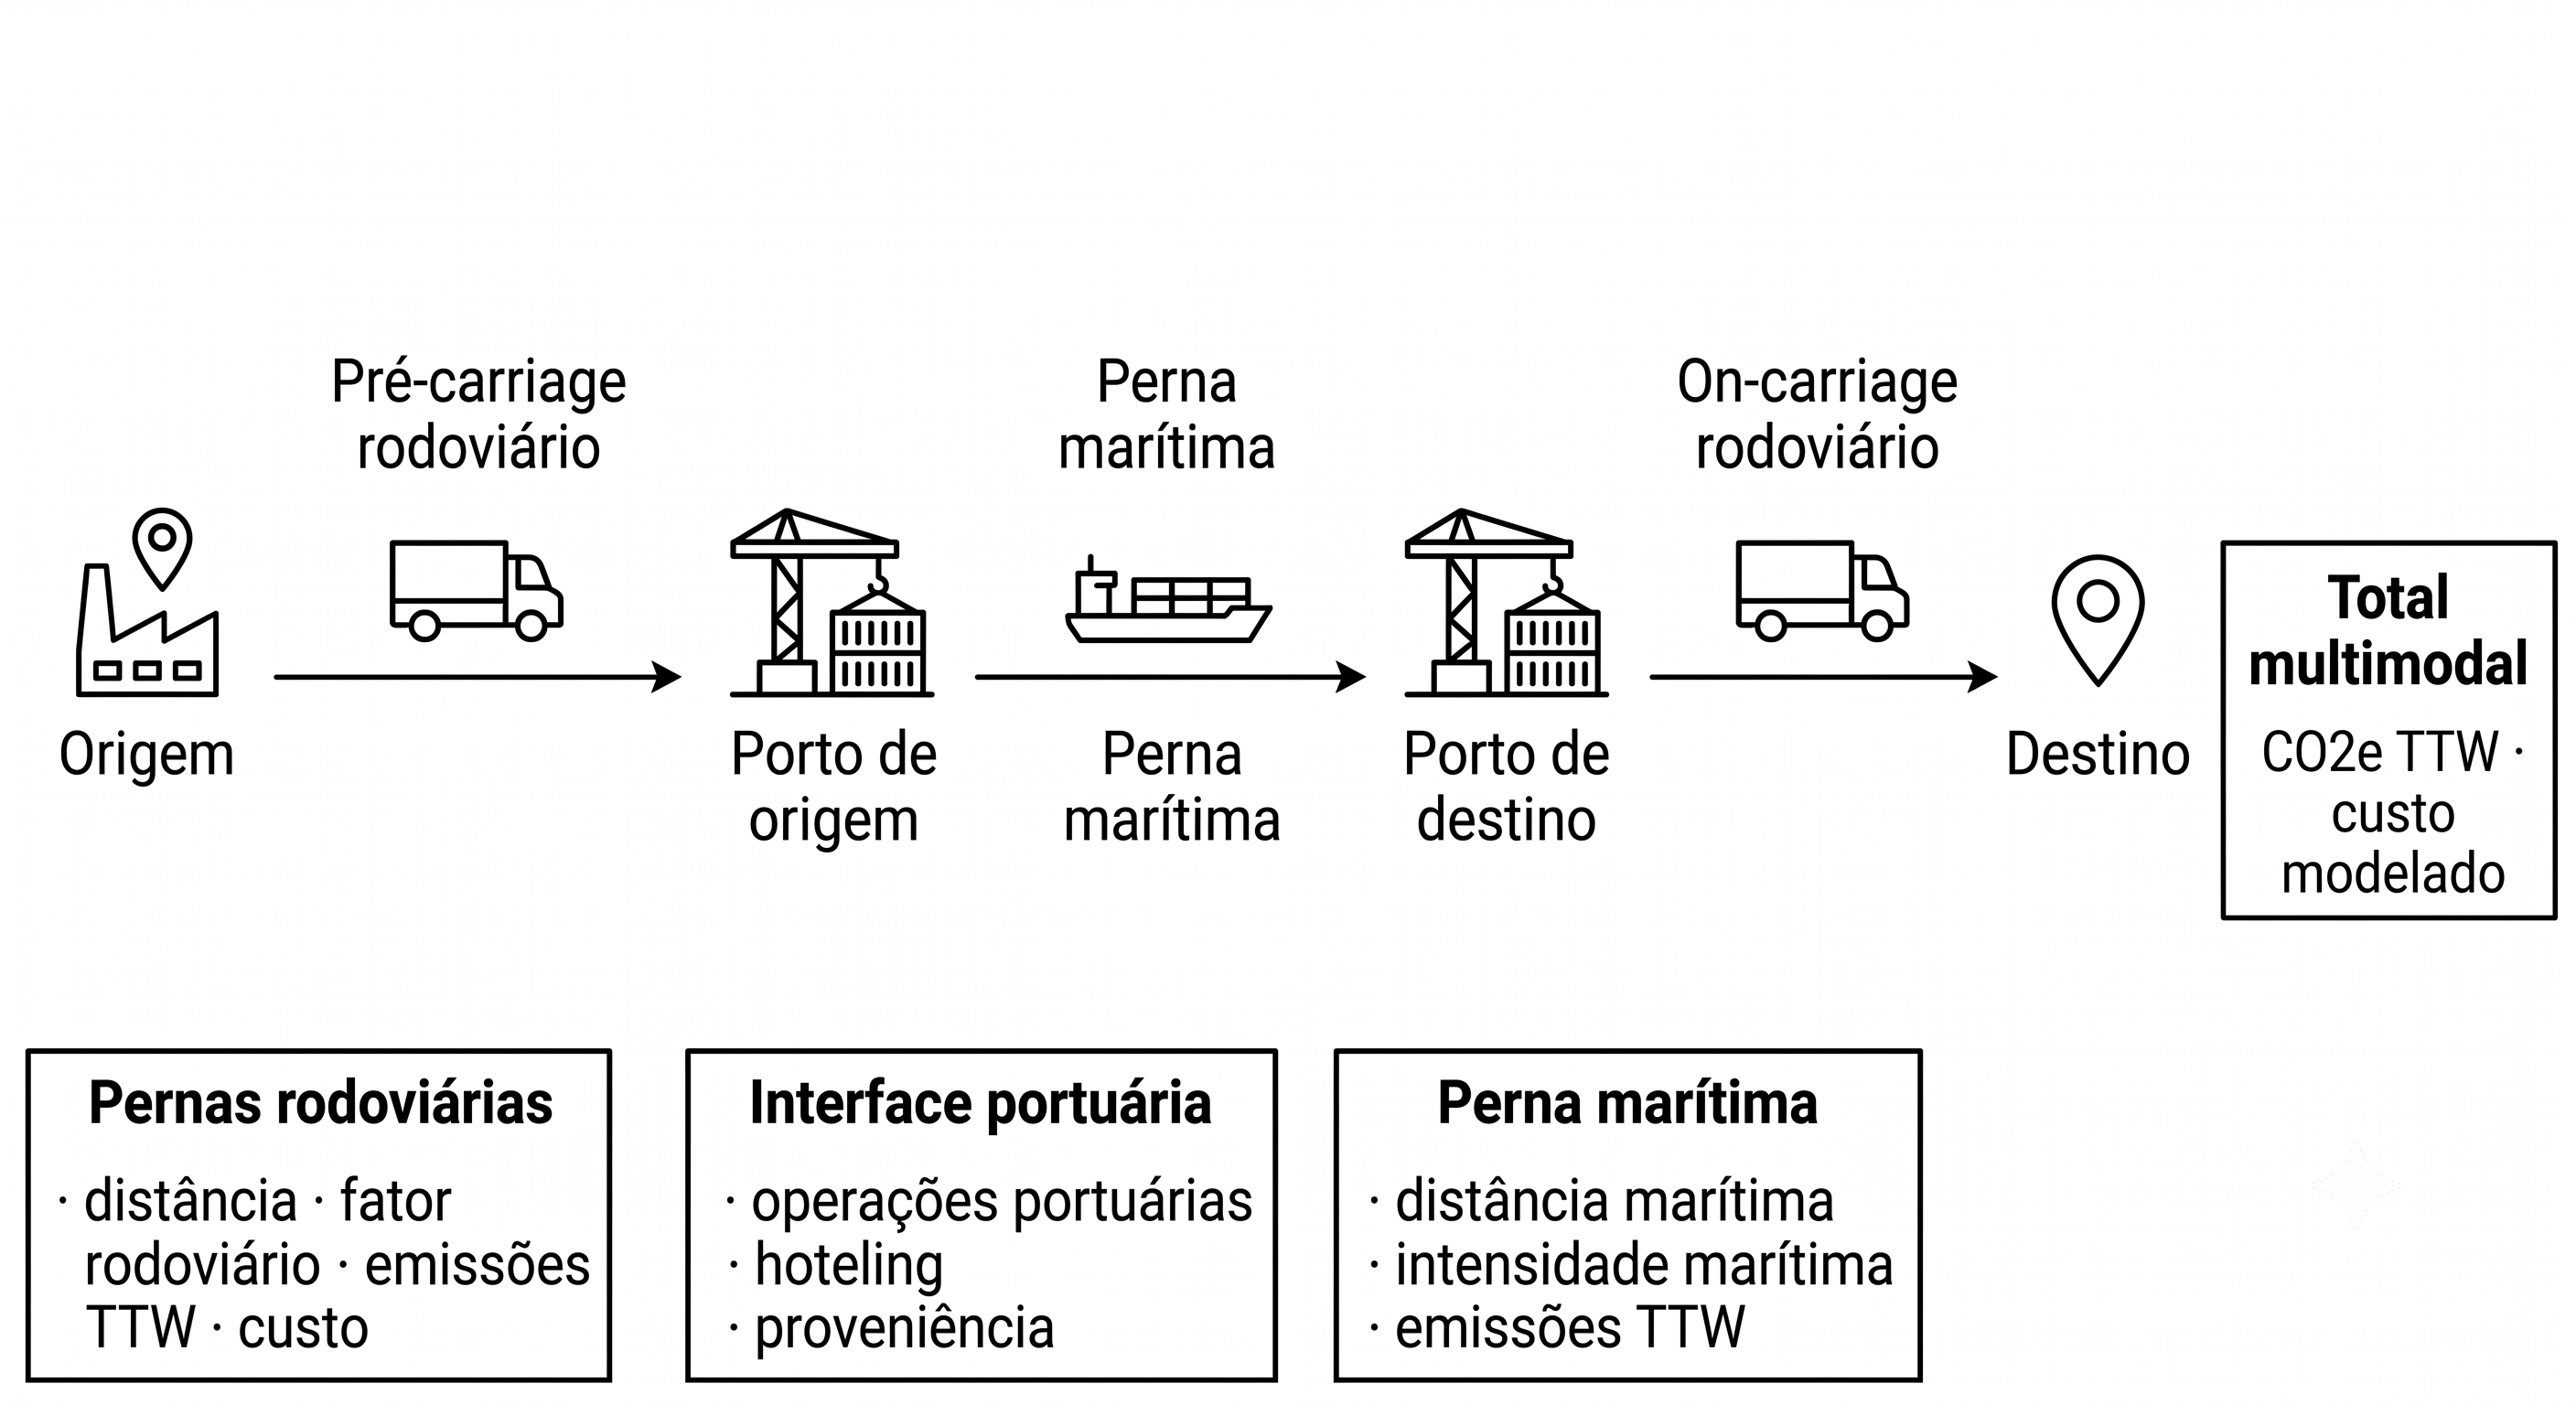
\includegraphics[width=0.95\textwidth]{images/figura_4_1.png}
\caption{Decomposição metodológica da alternativa multimodal em pernas rodoviárias, interface portuária, perna marítima e agregação final.}
\label{fig:cadeia-multimodal}
\end{figure}

A Figura~\ref{fig:cadeia-multimodal} evidencia a regra de agregação por componentes. O total multimodal não é a perna marítima isolada: é a soma dos acessos terrestres, da navegação e dos componentes portuários incluídos, cada um com distância, fator, custo e proveniência próprios.

\begin{equation}
R_{\mathrm{multi}} = R_{\mathrm{pre}} + R_{\mathrm{mar}} + R_{\mathrm{port}} + R_{\mathrm{on}}
\label{eq:multimodal-aggregation}
\end{equation}

Na Equação~\ref{eq:multimodal-aggregation}, \(R_{\mathrm{multi}}\) representa o resultado agregado da alternativa multimodal para uma dimensão de saída, como custo modelado ou emissões operacionais; \(R_{\mathrm{pre}}\) é o acesso rodoviário inicial; \(R_{\mathrm{mar}}\) é a perna marítima; \(R_{\mathrm{port}}\) representa operações portuárias e \emph{hoteling} incluídos; e \(R_{\mathrm{on}}\) é o acesso rodoviário final. A fórmula apenas explicita a composição do total e preserva a separação entre pernas.

\section{Reconstrução das viagens e formulação da intensidade marítima}
\label{sec:intensidade-maritima}

A estimativa marítima combina os registros de Carga e Atracação da ANTAQ com os indicadores de eficiência do EU MRV. A tabela de Carga registra movimentações associadas às escalas, incluindo massa, quantidade e portos relacionados à origem e ao destino da carga. A tabela de Atracação fornece a sequência temporal das escalas e o número IMO do navio. Depois da normalização dos nomes e códigos portuários, as escalas de cada viagem são ordenadas e chamadas consecutivas pertencentes ao mesmo complexo portuário são consolidadas sem descartar as movimentações de carga correspondentes.

Para um par de portos \((o,d)\), uma observação é elegível quando \(o\) aparece antes de \(d\) na sequência da mesma viagem. O procedimento examina todas as viagens elegíveis e todos os corredores observados entre o par, incluindo ligações diretas e percursos com uma ou mais escalas intermediárias. Não se impõe uma sequência fixa de portos. Se o mesmo par aparecer mais de uma vez dentro de uma viagem, mantém-se uma única observação dessa viagem para evitar dupla contagem; a escolha é determinística, priorizando a ocorrência direta e, na ausência dela, a de menor distância completa.

Seja \(\Delta m_{v,j}\) a movimentação líquida de massa na escala \(j\) da viagem \(v\), positiva para acréscimo líquido de carga a bordo e negativa para redução líquida. Como a janela observada pode começar com carga já embarcada, calcula-se uma carga inicial mínima que impeça valores negativos ao longo da sequência:

\begin{equation}
m_{v,0}=\max\left(0,-\min_k\sum_{j=1}^{k}\Delta m_{v,j}\right).
\label{eq:carga-inicial-maritima}
\end{equation}

A carga a bordo no subtrecho iniciado após a escala \(j\) é, então,

\begin{equation}
m_{v,j}=\max\left(0,m_{v,0}+\sum_{r=1}^{j}\Delta m_{v,r}\right).
\label{eq:carga-bordo-subtrecho}
\end{equation}

Essa reconstrução por saldo acumulado faz com que cada subtrecho use a massa efetivamente representada a bordo naquele ponto da viagem, em vez de atribuir a mesma carga a toda a sequência. Para a observação de \(o\) a \(d\), formada pelos subtrechos \(S_{v,o,d}\), o trabalho de transporte e o consumo de combustível alocado são dados por

\begin{equation}
\begin{aligned}
W_{v,o,d} &= \sum_{s\in S_{v,o,d}} m_{v,s}\,d_s, \\
F_{v,o,d} &= I_v\,W_{v,o,d}.
\end{aligned}
\label{eq:trabalho-consumo-viagem}
\end{equation}

em que \(d_s\) é a distância do subtrecho em milhas náuticas, \(W_{v,o,d}\) é expresso em \(\mathrm{t\,nm}\), \(I_v\) é a intensidade atribuída ao navio em \(\mathrm{g/(t\,nm)}\), e \(F_{v,o,d}\) é obtido em gramas. Assim, uma viagem com escalas intermediárias contribui pela soma de todos os subtrechos entre a origem e o destino, mantendo a carga a bordo e a distância próprias de cada um.

A intensidade \(I_v\) segue uma hierarquia de proveniência. A primeira opção é o valor positivo mais recente do EU MRV associado exatamente ao IMO observado na ANTAQ. Na ausência de correspondência, usa-se a estatística robusta da classe de embarcação, quando a classe está disponível; em seguida, usa-se a estatística do tipo de navio. Para o escopo conteinerizado, \emph{Container ship} é o tipo-padrão documentado quando o registro não oferece classificação mais específica. Se nenhuma etapa produz valor positivo, a intensidade da viagem permanece indisponível e essa ocorrência é contabilizada como não resolvida.

Os valores exatos por IMO são preservados sem corte, pois representam o indicador individual do navio. A regra de outliers aplica-se somente às estatísticas de fallback. Para o tipo de navio, os valores positivos mais recentes por IMO são ordenados e removem-se simetricamente \(\lfloor 0{,}01n\rfloor\) observações de cada cauda antes da média. Quando a amostra é pequena demais para retirar ao menos uma observação de cada lado, usa-se a mediana. Para a classe, utiliza-se a média aparada simétrica de 1\% em cada cauda registrada no artefato, operacionalizada pela exclusão dos valores abaixo do percentil 1 e acima do percentil 99; a mediana é usada quando essa estatística não está disponível. A fonte final registra o nível usado --- IMO, classe ou tipo --- e, nos fallbacks agregados, a estatística, o tamanho da amostra e a regra de outlier aplicável.

Uma única intensidade representativa é calculada para cada par ordenado de portos a partir de todas as observações de viagem com intensidade resolvida, sem restringir a amostra ao corredor escolhido para a geometria. Cada intensidade \(I_v\) recebe como peso o trabalho de transporte completo \(W_{v,o,d}\) da respectiva observação. A intensidade do par é a mediana ponderada, definida pela primeira intensidade na ordem crescente cuja soma acumulada dos pesos alcança 50\% do trabalho de transporte total:

\begin{equation}
I_{o,d}=\min\left\{x:\sum_{v:I_v\leq x}W_{v,o,d}\geq
\frac{1}{2}\sum_v W_{v,o,d}\right\}.
\label{eq:mediana-ponderada-intensidade}
\end{equation}

Observações com trabalho de transporte nulo não influenciam a Equação~\ref{eq:mediana-ponderada-intensidade} quando existe ao menos um peso positivo. Se todas as observações resolvidas do par tiverem trabalho nulo, adota-se a mediana não ponderada dessas intensidades e a fonte identifica explicitamente essa condição. A ausência de qualquer intensidade resolvida permanece indisponível, sem conversão para zero.

A estatística de intensidade e a escolha do caminho cumprem funções distintas. Todas as observações elegíveis com intensidade resolvida e trabalho positivo, distribuídas entre os diferentes corredores do par, alimentam a intensidade \(I_{o,d}\); o caminho usado no cenário é selecionado apenas para definir a sequência de portos e as distâncias navegadas. O critério geométrico prioriza um corredor direto observado e, entre alternativas da mesma categoria, a menor distância; sem corredor direto utilizável, escolhe-se o corredor multitrecho de menor distância. A intensidade observada do corredor selecionado é preservada como diagnóstico, mas não substitui a intensidade representativa do par.

Para uma remessa de massa \(m_{\mathrm{cen}}\), a navegação no cenário aplica \(I_{o,d}\) a cada distância do caminho selecionado:

\begin{equation}
F_{\mathrm{mar,cen}}=\frac{I_{o,d}\,m_{\mathrm{cen}}}{1000}
\sum_{s\in S_{\mathrm{sel}}}d_s,
\label{eq:combustivel-maritimo-cenario}
\end{equation}

em que o divisor converte gramas em quilogramas. Essa formulação mantém todos os corredores na estimação estatística, ao mesmo tempo que fornece uma geometria única e auditável para distância, combustível, custo modelado e emissões operacionais do cenário.

\section{Seleção de portos e definição de cenários}
\label{sec:selecao-portos}

A seleção de portos transforma a unidade funcional em uma cadeia multimodal concreta. Para uma mesma origem, destino e carga, diferentes portos podem alterar o comprimento do \emph{pre-carriage}, a distância marítima, o \emph{on-carriage}, os componentes portuários e a força da evidência disponível.

O método distingue três situações. Na seleção automática, portos elegíveis são escolhidos por uma lógica determinística e auditável dentro do conjunto configurado. Na seleção forçada ou manual, o cenário impõe porto de origem ou destino para representar uma hipótese específica, um benchmark ou uma análise controlada. Em cenários de sensibilidade, portos alternativos podem ser testados para avaliar como uma substituição declarada altera a comparação.

Essas situações não são intercambiáveis. Um porto selecionado para o caso-base, um porto forçado por hipótese e um porto alternativo de sensibilidade devem permanecer identificados como tal. Não há substituição silenciosa de um porto por outro: Pecém não valida Porto de Fortaleza, Suape não valida Porto do Recife, e um cenário alternativo não redefine automaticamente o cenário selecionado originalmente \cite{competitiveness2024,modalshiftreview2020}.

Essa seleção também não equivale a uma otimização comercial de rede. O método não resolve grade de navegação, frequência de escalas, disponibilidade de armador, slot, tempo de trânsito, confiabilidade, estoque em trânsito ou decisão de contratação. Esses elementos pertencem a uma fronteira de modelagem mais ampla.

\section{Proveniência das distâncias e hierarquia de confiança}
\label{sec:proveniencia-distancias}

A distância é um dos principais controles metodológicos do capítulo. Na alternativa rodoviária direta, ela define a perna origem-destino. Na alternativa multimodal, ela aparece separadamente no \emph{pre-carriage}, nos subtrechos do corredor marítimo selecionado e no \emph{on-carriage}. Por isso, dois cenários com totais calculados semelhantes podem ter força interpretativa diferente se a proveniência das distâncias for diferente. A origem da distância é registrada por subtrecho: usa-se primeiro um valor positivo da matriz marítima e, quando ele não existe para portos canônicos distintos, uma aproximação por coordenadas identificada como \texttt{haversine\_fallback}.

\begin{table}[htbp]
\centering
\small
\caption{Hierarquia de proveniência de distâncias.}
\label{tab:proveniencia-distancias}
\begin{tabularx}{\textwidth}{L{0.24\textwidth}Y Y}
\toprule
Proveniência & Uso metodológico & Limite de interpretação \\
\midrule
Roteamento rodoviário/cache & Distância modelada para pernas terrestres. & Não é trajetória GPS medida nem rota comercial efetivamente usada.\\
\texttt{seamatrix} & Distância marítima matricial para par de portos aplicável. & Não comprova escala, frequência, serviço ou contrato.\\
\texttt{external\_reference} & Referência documentada para o par de portos do cenário. & Só vale para o par e a unidade documentados.\\
\texttt{manual\_override} & Substituição explícita e rastreável para um cenário. & Exige motivação documentada; não deve ser generalizada.\\
\texttt{haversine\_fallback} & Estimativa geométrica quando falta distância marítima documentada. & Triagem ou lacuna de evidência; não valida rota marítima.\\
Referência ausente & Indica que a distância necessária não está suficientemente documentada. & Pode bloquear conclusão ou limitar o caso a sensibilidade.\\
\bottomrule
\end{tabularx}
\end{table}

Na Tabela~\ref{tab:proveniencia-distancias}, \texttt{seamatrix} e \texttt{external\_reference} oferecem evidência mais forte para a distância marítima porque representam uma matriz ou referência documentada para o par de portos. \texttt{manual\_override} pode ser adequado quando a substituição é explícita e justificada, mas sua validade fica restrita ao cenário. \texttt{haversine\_fallback} é útil para triagem quando falta referência marítima, porém tem menor força para conclusões numéricas. Essa hierarquia afeta a classificação da evidência; não altera, por si só, o fator de emissão ou a fronteira econômica.

\section{Cadeias conceituais de cálculo de emissões e custos}
\label{sec:cadeias-calculo}

Os cálculos são organizados como cadeias conceituais de transformação. Para cada perna rodoviária, a distância, a configuração de veículo e a carga definem o consumo estimado; o consumo e o fator implementado definem emissões operacionais \ttw{} de \cooe{}; o consumo e os insumos econômicos definem custo operacional modelado. Para a perna marítima, a intensidade representativa do par, a massa da remessa e as distâncias dos subtrechos selecionados definem o consumo de navegação conforme a Equação~\ref{eq:combustivel-maritimo-cenario}; esse consumo alimenta as emissões marítimas e o custo marítimo modelado.

Na alternativa rodoviária direta, há uma única cadeia de perna. Na alternativa multimodal, as cadeias do \emph{pre-carriage}, da perna marítima, dos componentes portuários e do \emph{on-carriage} são calculadas separadamente e depois agregadas. Essa decomposição preserva a distinção entre distância, consumo, custo e emissões, além de permitir que a proveniência de cada componente acompanhe o total.

Custos e emissões são dimensões metodológicas diferentes. O método pode mostrar que uma alternativa apresenta menor emissão, menor custo modelado, ambos, ou divergência entre essas dimensões. A interpretação exige que os componentes incluídos no total estejam declarados e que a comparação permaneça vinculada à mesma unidade funcional.

\section{Operações portuárias, hoteling e proveniência dos dados}
\label{sec:portops-metodologia}

Operações portuárias e \emph{hoteling} são tratados como componentes da cadeia multimodal quando incluídos na fronteira do cenário. Eles podem acrescentar consumo, emissões e custo modelado associados à permanência em porto, ao uso de sistemas auxiliares e às atividades de terminal. Sua inclusão depende de proveniência suficiente para indicar que tipo de componente foi representado, em qual porto ou condição, com qual unidade e sob qual fronteira \cite{berth2009,shipops2022,decarb2024}.

Quando há dado específico para o porto selecionado, o componente pode ser registrado como \texttt{observed}. Quando o dado específico não existe, a ausência não é interpretada como zero. O método usa uma hierarquia explícita: \texttt{estimated\_port\_average}, quando há média ponderada defensável de portos observados; \texttt{literature\_default}, quando há apenas um padrão documentado do modelo; ou \texttt{unavailable}, quando nenhum valor observado ou documentado pode ser atribuído.

A regra de consistência é evitar dupla contagem. Quando o cenário utiliza a intensidade MRV por trabalho de transporte, o indicador anual é tratado, para essa fronteira, como abrangente do consumo reportado do navio e o \emph{hoteling} não é acrescentado separadamente. As operações de terminal permanecem componentes explícitos quando têm proveniência representável. Nos modos em que navegação, permanência em porto e operação de terminal são modeladas separadamente, essa decomposição deve aparecer nos metadados e na interpretação do resultado.

\section{Qualidade de rota, classificação de evidências e limites de uso}
\label{sec:qualidade-evidencias}

A classificação de evidências é o mecanismo de controle de qualidade metodológica do TF. Antes de transformar um resultado calculado em argumento, o método verifica se a cadeia é comparável, se a distância tem proveniência suficiente, se os portos correspondem ao cenário declarado, se a fronteira ambiental e econômica foi preservada e se existem avisos como \emph{same-port}, \texttt{haversine\_fallback}, referência ausente ou porto alternativo.

\begin{table}[htbp]
\centering
\small
\caption{Classificações metodológicas usadas para controlar inferências.}
\label{tab:classificacoes-metodologia}
\begin{tabularx}{\textwidth}{L{0.28\textwidth}Y Y}
\toprule
Condição ou classificação & Significado metodológico & Uso seguro \\
\midrule
\codecell{observed\_input} & Registro de atividade com fonte, período e transformação identificados. & Reconstrução e auditoria dentro do recorte documentado.\\
\codecell{reference\_needed} & Falta evidência suficiente para distância ou premissa necessária. & Lacuna e prioridade de validação futura.\\
\codecell{excluded} & Caso inválido ou fora da fronteira adotada. & Justificativa de exclusão, sem uso numérico conclusivo.\\
\codecell{sensitivity\_only} / \codecell{sensitive} & Cenário ou resultado sob hipótese condicional. & Discussão condicionada, sem substituir caso-base.\\
\codecell{headline\_candidate} & Resultado com rota, fonte, unidade, fronteira e comparabilidade suficientes. & Uso como síntese principal somente dentro do escopo documentado.\\
\bottomrule
\end{tabularx}
\end{table}

A Tabela~\ref{tab:classificacoes-metodologia} antecipa a função da validação no Capítulo~\ref{ch:validacao}. Benchmarks externos, incluindo materiais associados ao Prof. Dr. Gustavo Costa, entram como comparação e diagnóstico de fronteiras. Eles podem apoiar uma leitura direcional ou revelar diferenças de premissa, mas não redefinem o caso-base, não calibram magnitudes sem alinhamento metodológico completo e não transformam custo modelado em frete comercial.
